\documentclass[11pt,a4paper]{article}
\usepackage[T1]{fontenc}
\usepackage[utf8]{inputenc}
\usepackage{lmodern}
\usepackage{microtype}
\usepackage{amsmath,amssymb,amsthm,mathtools,bm}
\usepackage{booktabs,array,tabularx,longtable}
\usepackage{graphicx,float,caption}
\usepackage{xcolor}
\usepackage[margin=2.15cm]{geometry}
\usepackage{enumitem}
\usepackage{fancyhdr}
\usepackage[hidelinks,pdfencoding=auto]{hyperref}

\hypersetup{
  pdftitle={FIN ST248--ST262: Preparation-Source Obstructions, an Affine Carrier Connection, and Log-Haar Refinement},
  pdfauthor={Krzysztof Żuchowski},
  pdfsubject={Analytical, interval, exact, and computational execution of FIN programs ST248--ST262},
  pdfkeywords={FIN, fractal information, selector obstruction, equivariant operators, affine connection, Krawczyk continuation, quantum recovery, HMM transfer operator, graph refinement, spectral dimension, Haar measure}
}

\definecolor{proved}{RGB}{20,92,48}
\definecolor{conditional}{RGB}{148,88,0}
\definecolor{blocked}{RGB}{150,28,28}
\newcommand{\Proven}{\textcolor{proved}{\textbf{[PROVEN]}}}
\newcommand{\Evidence}{\textcolor{conditional}{\textbf{[STRONG NUMERICAL EVIDENCE]}}}
\newcommand{\Conditional}{\textcolor{conditional}{\textbf{[CONDITIONAL]}}}
\newcommand{\Blocked}{\textcolor{blocked}{\textbf{[BLOCKED]}}}
\newcommand{\R}{\mathbb R}
\newcommand{\C}{\mathbb C}
\newcommand{\Tr}{\operatorname{tr}}
\newcommand{\diag}{\operatorname{diag}}
\newtheorem{theorem}{Theorem}[section]
\newtheorem{proposition}[theorem]{Proposition}
\newtheorem{corollary}[theorem]{Corollary}

\pagestyle{fancy}
\fancyhf{}
\lhead{FIN ST248--ST262}
\rhead{Release 10.74}
\cfoot{\thepage}
\setlength{\headheight}{14pt}
\setlist[itemize]{leftmargin=1.3em,itemsep=2pt,topsep=3pt}
\setlist[enumerate]{leftmargin=1.5em,itemsep=2pt,topsep=3pt}
\sloppy

\begin{document}
\hypersetup{pageanchor=false}
\begin{titlepage}
\centering
\vspace*{1.0cm}
{\Large Fractal Information Theory Project\par}
\vspace{0.9cm}
{\huge\bfseries FIN ST248--ST262\par}
\vspace{0.4cm}
{\LARGE Preparation-Source Obstructions,\par}
{\LARGE an Affine Carrier Connection, and Log-Haar Refinement\par}
\vspace{1.0cm}
{\large Analytical, interval, exact, and computational research report\par}
\vfill
{\Large Krzysztof \.{Z}uchowski\par}
\vspace{0.2cm}
{\large Independent Researcher --- Fractal Information Theory Project\par}
{\large ORCID: 0009-0002-0909-3613\par}
\vspace{0.8cm}
{\large August 12, 2026\par}
\vspace{0.3cm}
{\large Release 10.74\par}
\vfill
\begin{minipage}{0.92\textwidth}
\small
\textbf{Repository snapshot.} The audited tracked base is commit
\texttt{10d0ccc19ac7b9101c7d382dd0859b352cec802f}. The working tree contains
uncommitted and untracked research artifacts. Reproduction therefore depends on the
source-packet hashes in the accompanying SHA-256 manifest, not on the tracked commit alone.

\medskip
\textbf{License.} CC BY 4.0. \quad \textbf{Language.} English. \quad
\textbf{Resource type.} Preprint and executable reproducibility package.
\end{minipage}
\end{titlepage}
\hypersetup{pageanchor=true}
\pagenumbering{roman}

\begin{abstract}
Programs ST248--ST262 test whether the state, connection, refinement, and scale-flow
objects identified in Release 10.73 can be generated or reduced further. ST248 proves a
sharp obstruction: every deterministic $D_{12}$-natural probability state constructed from
the strict operator $A$ alone is uniform. Therefore the localized state used in
$M_\rho=\diag\rho$ cannot be hidden inside an equivariant function of $A$. ST249 then
classifies all linear $D_{12}$-equivariant vertex-state processors as the seven-dimensional
distance algebra and proves that they can preserve or erase, but cannot create, selector
information absent from their input state.

Several positive closures follow. ST250 certifies 360 additional pseudo-arclength boxes,
giving eight local steps on every signed branch. ST251 proves the exact global recovery
optimum $81/100$ for a rational, fully non-diagonal, nonunital rotated amplitude-damping
channel. ST253 proves that $A$ induces a positive metric and a canonical flat Levi-Civita
connection on the mean-zero affine amplitude carrier; this connection cancels the
nonlinear chart artifact found in ST239. ST254 certifies every one of $28^3=21{,}952$
nuisance boxes at halfwidth $0.0005$. ST255 constructs an exactly finite-sample efficient
modal estimator. ST257 gives a direct outward belief-transfer spectral-radius enclosure
and improves the certified Hellinger-rate interval after intersection with the independent
previous bound.

At the refinement frontier, graph-Laplacian locality reduces the abstract 78-dimensional
two-child moduli space to a seven-dimensional positive cone but does not select one member.
Complement-resolving preparations and effects reconstruct the hidden generator exactly,
whereas every coarse experiment is blind to it. Finally, ST260 proves that the unique
scale-invariant rate measure is the log-Haar measure $\rho\,d\mu/\mu$ and that it contributes
the constant $2\rho\ln2$ to spectral dimension. This gives a precise mathematical form to
a fractal-layer plateau, but its density, cutoffs, realization, and physical units remain
additional data. No selector closure, dimensional physics, laboratory evidence,
legacy-to-strict role transfer, Standard Model, gravity, or Theory-of-Everything closure is
claimed.
\end{abstract}

\tableofcontents
\newpage
\pagenumbering{arabic}

\section{Executive conclusions}

The research batch yields four structural conclusions.

\begin{enumerate}
\item \textbf{The preparation obstruction is exact.} If the only input is the fully
$D_{12}$-symmetric strict operator, deterministic naturality forces the output probability
state to be uniform. A localized state requires a boundary, an orbit label, a random
realization, or a genuinely new symmetry-breaking object.
\item \textbf{A nonlinear response connection exists conditionally.} On the canonical
mean-zero affine amplitude carrier, $A$ is a positive metric and its Levi-Civita connection
is flat and natural. This solves nonlinear chart transport mathematically inside that
carrier, but it is not a spacetime or gauge connection.
\item \textbf{Locality reduces refinement freedom without removing it.} Exact coarse
diffusion plus graph-Laplacian signs and the declared symmetries leave six independent edge
splits and one vertical rate.
\item \textbf{A fractal plateau has a unique scale-invariant measure.} The positive
multiplicative group has Haar measure $d\mu/\mu$, and its integrated fiber contribution is
independent of time. What is missing is no longer the mathematical shape of the plateau,
but a strict source for its density, cutoffs, and operational realization.
\end{enumerate}

Thus the deepest surviving statement is
\begin{align*}
A&\text{ determines symmetric dynamics and a quotient geometry},\\
A&\text{ does not determine a localized state or a unique refinement}.
\end{align*}

\section{Scope, kernel discipline, and proof labels}

The strict working object remains
\[
A=sI-W,\qquad W_{xx}=0,\qquad
W_{xy}=K_{\rm strict}(d(x,y))\quad(x\ne y),
\]
with $A\bm1=0$ and $A\succeq0$. The diagonal exclusion is part of the definition. The
historical $K_{\rm legacy,ont}$ remains an intermediate bridge kernel; it is not silently
identified with $K_{\rm strict}$, and no legacy physical-role formula is transferred.

The project ontology treats the nadsoliton itself as primordial fractal information in a
solitonic state. The present report analyzes mathematical consequences of a finite strict
operator. It does not infer that a physical universe, matter, or spacetime has been derived.

\begin{itemize}
\item \Proven{} means an exact deduction or a finite outward certificate within its stated
class.
\item \Evidence{} means a reproducible numerical result without an exact or interval
global-optimality proof.
\item \Conditional{} means that the stated carrier, state, control cost, channel class, or
scale measure is an explicit premise.
\item \Blocked{} means that the needed evidence or source object is absent.
\end{itemize}

\section{Program ledger}

\small
\begin{longtable}{@{}>{\bfseries}p{0.07\textwidth}p{0.24\textwidth}p{0.31\textwidth}p{0.21\textwidth}@{}}
\toprule
Program & Object & Result & Boundary\\
\midrule
\endhead
ST248 & Preparation source & \Proven{} deterministic $D_{12}$-natural no-go & New symmetry-breaking classes remain\\
ST249 & Typed second operators & \Proven{} seven-dimensional linear classification & Nonlinear maps open\\
ST250 & Branch extension & \Proven{} 360 new local boxes & Explicit finite stop\\
ST251 & Nonunital recovery & \Proven{} global optimum $81/100$ & Rotated amplitude damping class\\
ST252 & Selector ledger & \Evidence{} feasible augmented cost $0.440546$ & No interval KKT certificate\\
ST253 & Carrier connection & \Conditional{} flat Levi-Civita completion & Affine amplitude carrier supplied\\
ST254 & Nuisance cover & \Proven{} 21,952/21,952 boxes & Not a maximal domain\\
ST255 & Mode estimator & \Proven{} exact finite-sample efficiency & Declared local multinomial model\\
ST256 & Joint Clifford pair & \Proven{} aligned two-gap uniqueness & Generic misalignment open\\
ST257 & HMM transfer & \Proven{} outward spectral-radius enclosure & Fixed $s=1/2$ HMM\\
ST258 & Thermal reset & \Proven{} ideal pulse and Gibbs error law & Controller and physical units supplied\\
ST259 & Local refinement & \Proven{} seven-dimensional positive cone & No member selected\\
ST260 & Scale plateau & \Conditional{} exact log-Haar theorem & Density and cutoffs unsourced\\
ST261 & Refinement observables & \Proven{} coarse no-go and complement tomography & Fiber instrument not supplied\\
ST262 & External evidence & \Blocked{} & No independent laboratory record\\
\bottomrule
\end{longtable}
\normalsize

\section{ST248--ST249: where the selector information must enter}

\subsection{The strict preparation-source no-go}

Let $F$ be a deterministic rule assigning a probability vector to a self-adjoint vertex
operator, and impose naturality
\[
F(gAg^{-1})=gF(A),\qquad g\in D_{12}.
\]
The strict $A$ is fixed by every $g$. Therefore $F(A)=gF(A)$ for the complete transitive
action. The only invariant probability vector is $\bm1/12$.

\begin{theorem}[No localized state from symmetric $A$ alone]
No deterministic $D_{12}$-natural state-valued function of $A$ can generate the localized
state required by the noncommuting multiplication operator $M_\rho$.
\end{theorem}

The diagonals of $e^{-0.7A}$, $(I+A)^{-1}$, and $A^2$, after normalization, replay the
theorem numerically to errors below $3\times10^{-16}$. By contrast,
$e^{-0.7A}\delta_0$ lies $0.323238$ from uniform and gives
$\|[A,M_\rho]\|_F=0.265194$. The difference is exactly the supplied preparation
$\delta_0$.

\begin{figure}[H]
\centering
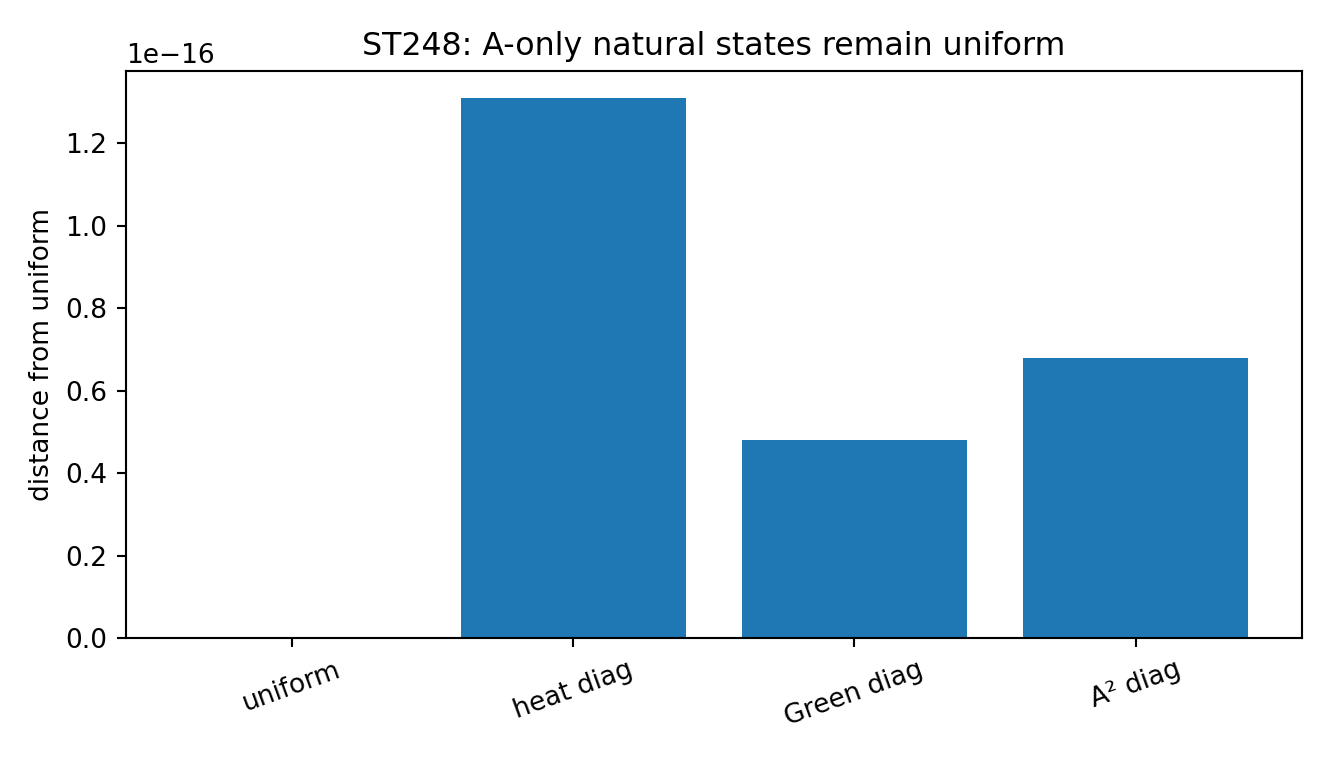
\includegraphics[width=.79\textwidth]{FIN_ST248_ST262_Figures/st248_preparation_no_go.png}
\caption{ST248: state candidates generated without an orbit label remain uniform.}
\end{figure}

This is a no-go for a declared class, not for spontaneous stochastic realization or a new
strict symmetry-breaking field. QW-2191 remains open.

\subsection{Complete linear typed-operator classification}

The vertex permutation representation of $D_{12}$ decomposes multiplicity-free into seven
real distance sectors. Hence every linear equivariant state processor is
\[
C=\sum_{d=0}^{6}c_dB_d,
\]
where $B_d$ is the distance-$d$ adjacency matrix. Positivity and mass preservation cut out
the affine Markov polytope. Every typed multiplication operator in this class is
\[
\rho\longmapsto M_{C\rho}=\diag(C\rho).
\]

Equivariance implies
\[
\operatorname{Stab}(\rho)\subseteq\operatorname{Stab}(C\rho).
\]
Thus processing may erase asymmetry but cannot create orbit information absent from the
condition. Uniform, even-localized, and chiral inputs yield stabilizer orders $24$, $2$,
and $1$, respectively. The chiral state is the minimal orbit type in this class capable of
carrying both localization and orientation.

\section{ST250: bounded continuation of every signed branch}

Starting from the two-step endpoints of ST236, six further pseudo-arclength correctors were
validated for each of sixty signed seeds. All $360/360$ new boxes pass. Every complete seed
now has eight certified steps. The minimum new rank margin remains positive, and the
minimum clearance between boxes from different exact fold pairs is
\[
0.0094481743.
\]
No nonfold intersections occur in the traced extension, so the finite incidence graph still
has thirty components.

\begin{figure}[H]
\centering
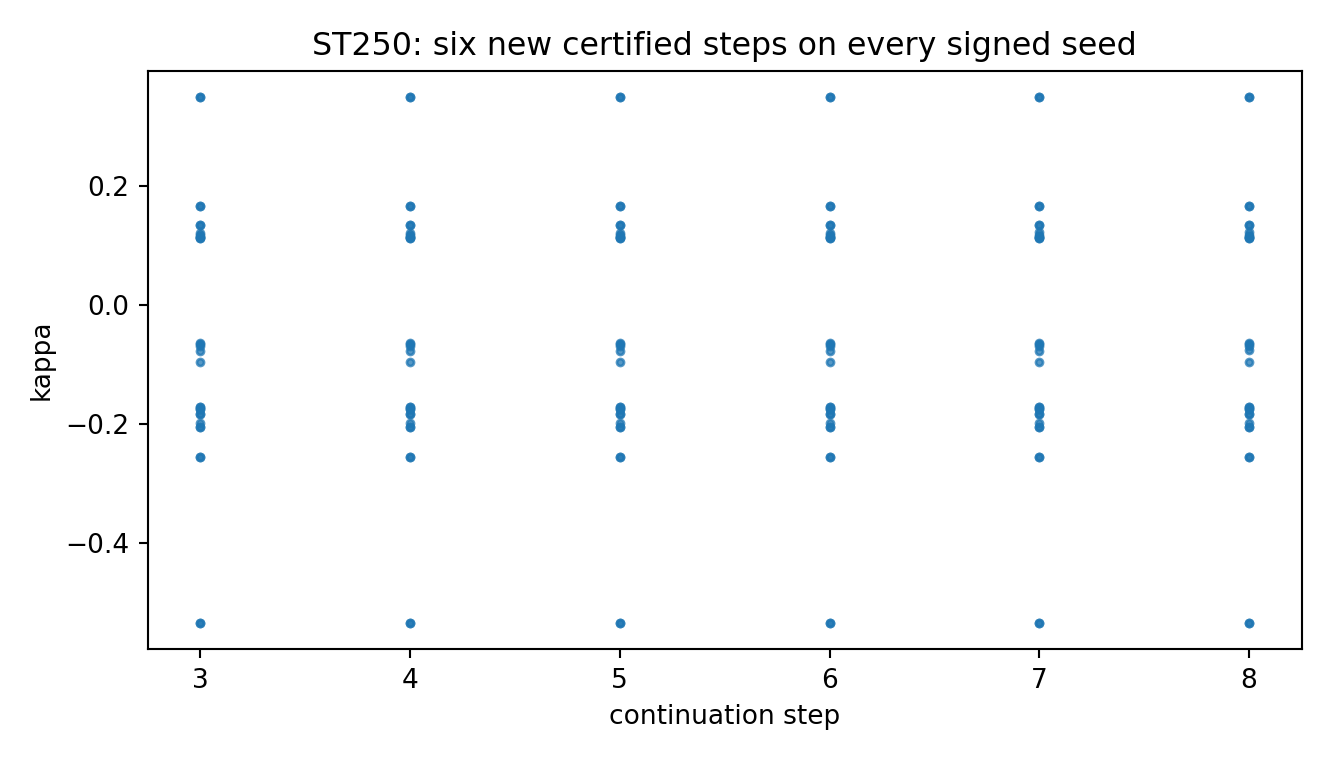
\includegraphics[width=.83\textwidth]{FIN_ST248_ST262_Figures/st250_branch_extension.png}
\caption{ST250: six new outward-certified steps on every signed seed.}
\end{figure}

The stop after six new steps is explicit. Nothing here excludes a later collision,
secondary bifurcation, or distant connection, and the branches are not identified with
physical particles.

\section{ST251: a fully non-diagonal nonunital recovery theorem}

Take amplitude damping with rational Kraus operators
\[
K_0=\begin{pmatrix}1&0\\0&4/5\end{pmatrix},\qquad
K_1=\begin{pmatrix}0&3/5\\0&0\end{pmatrix},
\]
and compose it with rational pre- and post-unitaries
\[
U=\frac15\begin{pmatrix}3&4\\-4&3\end{pmatrix},\qquad
V=\frac1{13}\begin{pmatrix}5&12\\-12&5\end{pmatrix}.
\]
The resulting affine Bloch map is nonunital and has off-diagonal linear norm $0.892378$.

\begin{theorem}[Global CPTP optimum]
The optimal recovery over every CPTP qubit map is
\[
R=U^*V^*=\frac1{65}\begin{pmatrix}-33&-56\\56&-33\end{pmatrix},
\qquad F_e^*=\frac{81}{100}.
\]
\end{theorem}

For the base damping channel, the exact dual is
\[
Y=\diag(9/20,9/25).
\]
Its trace is $81/100$, and the slack consists of two positive scalar blocks and
$\frac15\left(\begin{smallmatrix}1&-1\\-1&1\end{smallmatrix}\right)$. Rational unitary
transport gives the displayed channel primal and dual with zero exact gap. This extends the
previous Pauli and replacer families, but not all affine channels.

\section{ST252: endpoint and actuator costs}

The ST238 two-state selector model was augmented by ten control knots, a hard dimensionless
slew bound $|\dot\pi|\le0.30$, a quadratic actuator term, and endpoint KL costs relative to
the baseline state. The ledger is
\[
J=\Sigma_{\rm Markov}+J_{\rm slew}+J_{\rm endpoints}.
\]
Three independent starts converge to values agreeing within $3\times10^{-13}$. The best
feasible schedule gives
\begin{align*}
J&=0.4405461745, & \Sigma&=0.3347718379,\\
J_{\rm slew}&=0.0054698773, & J_{\rm endpoints}&=0.1003044593.
\end{align*}
The final-state residual is $1.2\times10^{-14}$, and the slew constraint is active.

\begin{figure}[H]
\centering
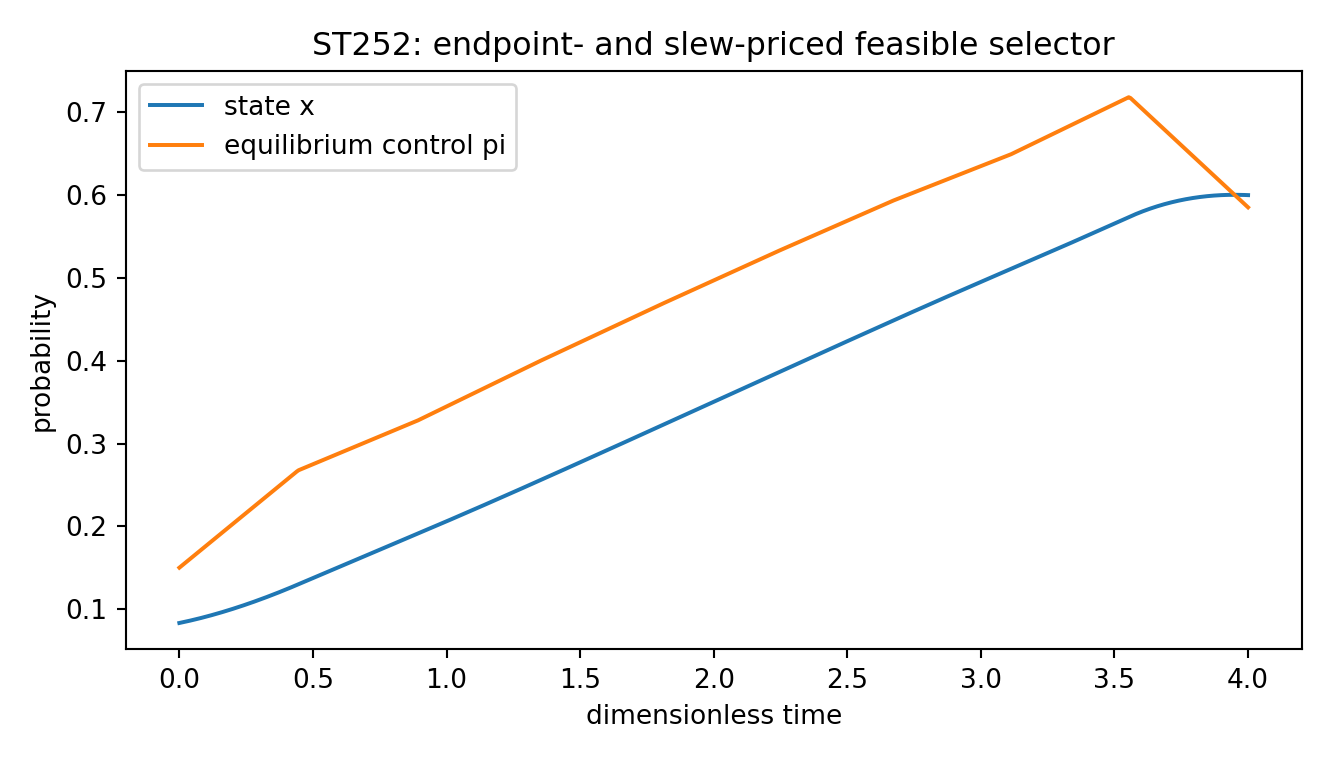
\includegraphics[width=.82\textwidth]{FIN_ST248_ST262_Figures/st252_actuator_selector.png}
\caption{ST252: a feasible selector path after endpoint and finite-rate actuator pricing.}
\end{figure}

All added costs are nonnegative, so the verified ST238 lower bound $0.3176910887$ remains
a rigorous lower bound. The new schedule is only a numerical upper bound; without an
interval KKT certificate, global optimality is not claimed. None of the coefficients are
physical joules.

\section{ST253: the mean-zero affine carrier connection}

Because $\ker A=\operatorname{span}\bm1$, the strict operator induces a positive metric on
\[
H_0=\{\psi\in\R^{12}:\bm1^T\psi=0\},\qquad
g_A(u,v)=u^TAv.
\]
The metric eigenvalues lie between $0.754121$ and $2.342182$. On the affine vector space
$H_0$, the translation-invariant metric has a unique Levi-Civita connection. It is
$D_{12}$-invariant, flat, and torsion-free.

The nonlinear scalar audit uses $x=y+cy^6$ and
\[
V(x)=\frac a2x^2+\frac g{12}x^{12}.
\]
Ordinary differentiation gives
\[
\frac{D_y^{12}V}{11!}=g+6ac^2.
\]
Transporting the flat connection gives $\Gamma_y=x''/x'$ and the recursion
\[
T_{k+1}=\partial_yT_k-k\Gamma_yT_k.
\]
Exact symbolic evaluation yields
\[
\frac{\nabla_y^{12}V}{11!}=g.
\]
The chart artifact cancels exactly.

This is a meaningful completion of ST239, conditional on the affine mean-zero amplitude
carrier. It is not a physical spacetime, gravitational, or gauge connection.

\section{ST254: complete nuisance-cover extension}

The cube centered at $(0.2,0.7,0.05)$ with halfwidth $0.0005$ was tiled by
$28^3=21{,}952$ closed boxes. Every outward Krawczyk test passes. The minimum inclusion
margin is
\[
1.4721098531\times10^{-4},
\]
and the maximum is $2.0794075222\times10^{-4}$. This converts the sampled ST240 diagnosis
into a complete cube theorem.

\begin{figure}[H]
\centering
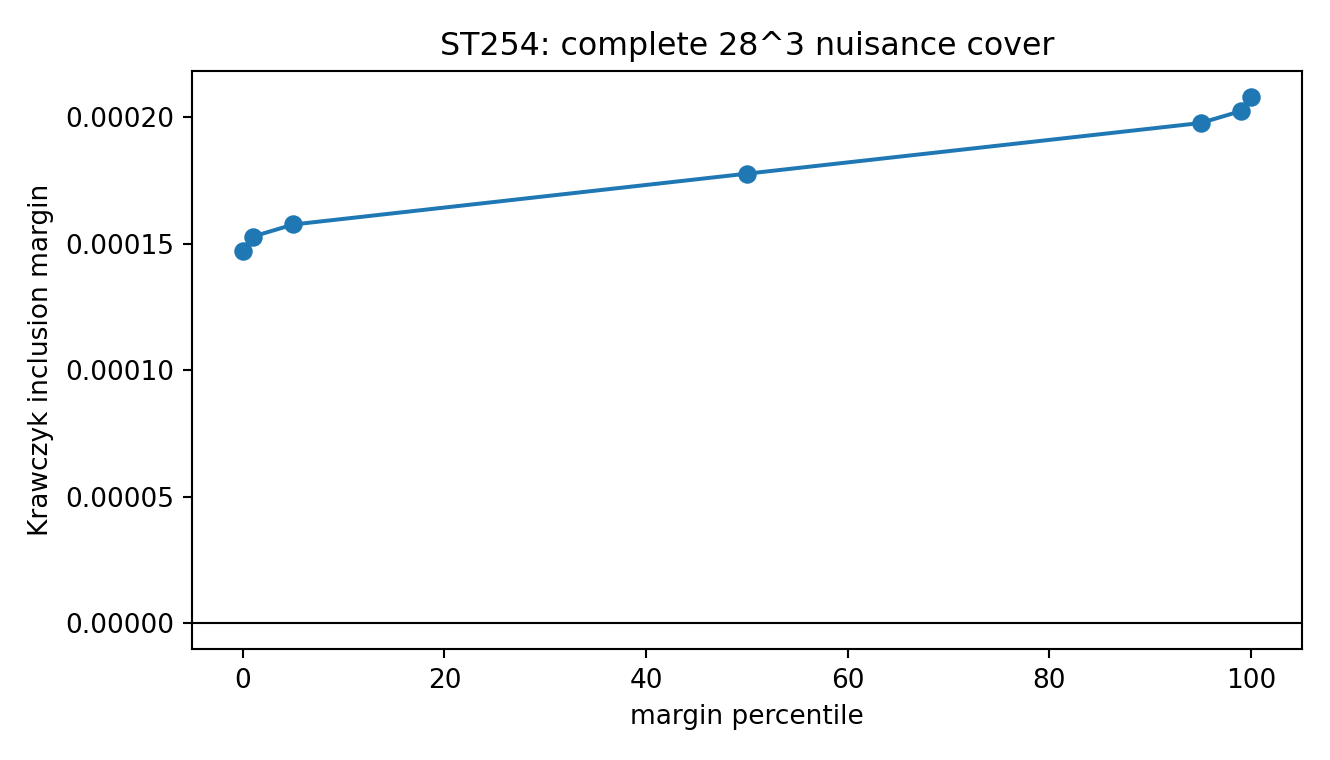
\includegraphics[width=.82\textwidth]{FIN_ST248_ST262_Figures/st254_cover_margins.png}
\caption{ST254: inclusion-margin percentiles over the complete $28^3$ cover.}
\end{figure}

The result is a continuation domain, not an experimental tolerance or a proof that the
domain is maximal.

\section{ST255--ST257: exact estimation and transfer-operator inference}

\subsection{Finite-sample efficient modal estimators}

For orthonormal mean-zero Fourier modes $v_k$ and attenuations $\sigma_k$, consider the
local multinomial family
\[
p(\theta)=\frac{\bm1}{12}+\sum_{k=1}^{6}\sigma_k\theta_kv_k.
\]
The estimator
\[
\widehat\theta_k=\frac{v_k^T(\widehat p-\bm1/12)}{\sigma_k}
\]
is exactly unbiased wherever the probabilities are nonnegative. At the uniform state,
\[
\operatorname{Cov}(\widehat\theta)=
\diag\left(\frac1{12n\sigma_k^2}\right)=\frac{I^{-1}}n.
\]
It attains the finite-sample Cram\'er--Rao matrix exactly. In the supplied common-shock
cluster model, the covariance is multiplied exactly by $1+(20-1)0.05=1.95$.

\begin{figure}[H]
\centering
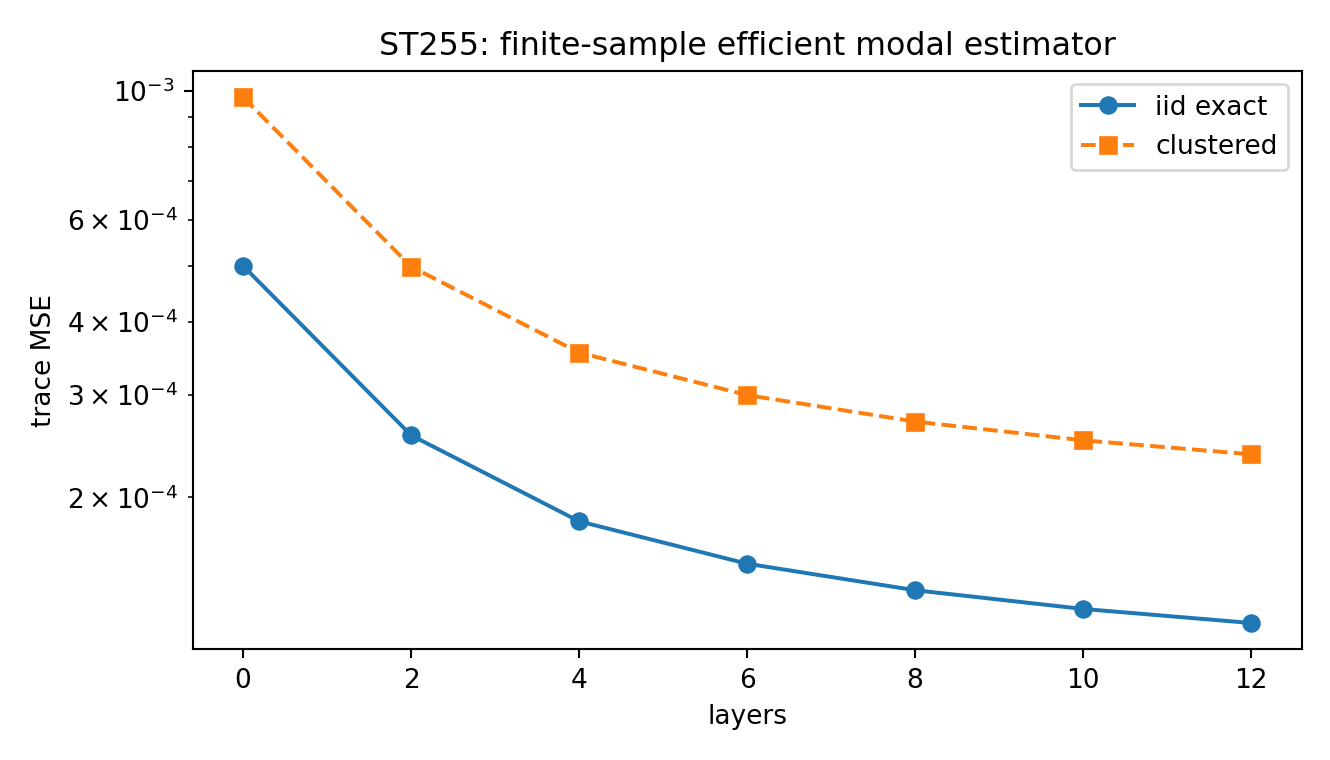
\includegraphics[width=.81\textwidth]{FIN_ST248_ST262_Figures/st255_estimators.png}
\caption{ST255: exact trace MSE and cluster inflation across developed layers.}
\end{figure}

\subsection{An aligned two-gap Clifford theorem}

Let $(X_*,Z_*)$ be any balanced Hermitian Clifford pair and let
\[
X_0=\alpha X_*,\qquad Z_0=\beta Z_*,\qquad \alpha,\beta>0.
\]
For every competing Clifford pair,
\[
\Delta J=\alpha\|X-X_*\|_F^2+\beta\|Z-Z_*\|_F^2.
\]
Thus $(X_*,Z_*)$ is the unique global joint minimizer in every balanced dimension. This is
an exact global theorem for the aligned two-gap class and is invariant under common unitary
conjugation. Marginal sign gaps alone for arbitrary misaligned targets are not settled.

\subsection{Direct belief-transfer spectral radius}

For the observed HMM, define the positive transfer operator
\[
(Tf)(b_0,b_1)=\sum_y\sqrt{q_{0,y}(b_0)q_{1,y}(b_1)}
f(F_{0,y}(b_0),F_{1,y}(b_1)).
\]
Adjacent floating intervals enclose every exact decimal parameter. A $24^2$ cover of the
complete belief square and depth-nine outward recursion give
\[
T^9\bm1\in[0.00058633896,0.00166319692].
\]
For a positive operator, $m\bm1\le T^n\bm1\le M\bm1$ implies
\[
m^{1/n}\le r(T)\le M^{1/n}.
\]
Hence
\[
r(T)\in[0.43742683,0.49115206],qquad
\mathcal C_{1/2}\in[0.71100152,0.82684584].
\]
Intersecting with the independent previous certificate yields
\[
\boxed{\mathcal C_{1/2}\in[0.7110015196,0.8198470893]},
\]
of width $0.10884557$. This is a direct interval transfer result, not the strong-numerical
Chernoff optimization of ST243.

\section{ST258: ideal controller pulse and finite-temperature blanks}

For two identical registers let $S$ denote global SWAP and choose
\[
H_c=\frac{\pi}{2\tau}(I-S),\qquad 0<t<\tau.
\]
Then
\[
e^{-i\tau H_c}=S,qquad [H_c,H_{\rm total}]=0.
\]
The expectation of $H_c$ is constant during the pulse, so ideal sudden switching on and off
has zero net closed-system work. This does not include dissipation in a finite controller.

A Gibbs blank with dimensionless gap $\beta\epsilon$ has residual reset error
\[
\delta=\frac1{1+e^{\beta\epsilon}},\qquad
\beta\epsilon=\log\frac{1-\delta}{\delta}.
\]
Exact pure reset requires $\beta\epsilon\to\infty$. The blank is therefore a thermodynamic
resource rather than a free logical symbol.

\begin{figure}[H]
\centering
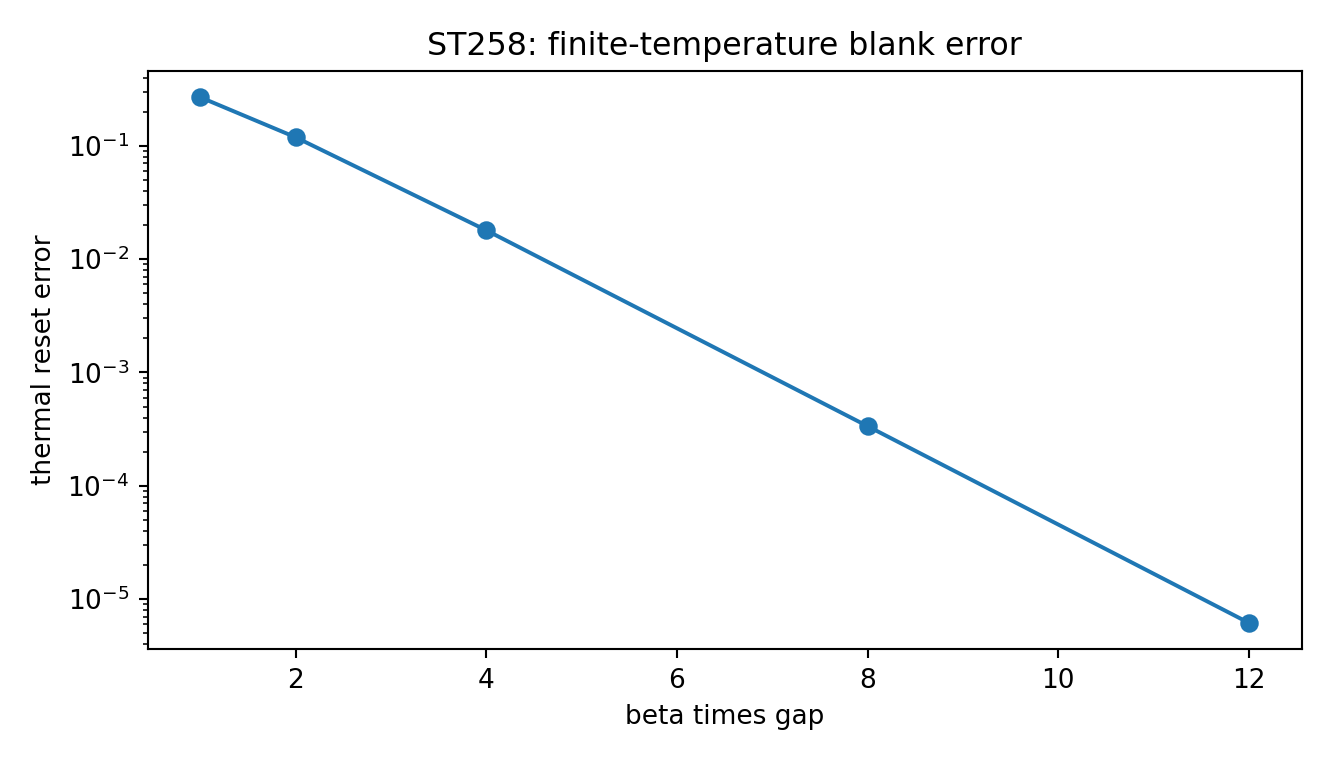
\includegraphics[width=.78\textwidth]{FIN_ST248_ST262_Figures/st258_thermal_blank.png}
\caption{ST258: finite-temperature reset error as a function of the dimensionless gap.}
\end{figure}

\section{ST259: the local positive refinement cone}

Label refined vertices by $(i,a)$ with base vertex $i\in\mathbb Z_{12}$ and fiber
$a\in\{0,1\}$. Let $p_d$ be the same-fiber weight, $q_d$ the cross-fiber weight at base
distance $d$, and $v$ the vertical weight. Translation, reflection, and fiber swap leave
these parameters invariant.

\begin{theorem}[Local graph-Laplacian classification]
The refined graph Laplacian exactly intertwines the coarse strict generator if and only if
\[
p_d\ge0,\quad q_d\ge0,\quad p_d+q_d=W_d\quad(d=1,\ldots,6),
\qquad v\ge0.
\]
\end{theorem}

Thus the 78-dimensional abstract symmetric complement cone collapses to six closed
intervals times one ray. All sampled matrices have nonpositive off-diagonals, zero row sum,
positive spectrum, and intertwining error below $2.1\times10^{-15}$. If same- and
cross-fiber edges are declared indistinguishable, $p_d=q_d=W_d/2$ and only $v$ remains.
Neither symmetry nor locality chooses the remaining parameters.

\section{ST260: the log-Haar plateau theorem}

Each two-state fiber gap $\mu$ contributes
\[
f(\mu t)=\frac{4\mu t}{e^{2\mu t}+1}
\]
to spectral dimension. Exact invariance under scale multiplication selects, up to a
constant density $\rho$, the Haar measure of $\R_{>0}$:
\[
d\nu(\mu)=\rho\frac{d\mu}{\mu}.
\]

\begin{theorem}[Scale-invariant plateau]
For every $t>0$,
\[
\int_0^\infty \frac{4\mu t}{e^{2\mu t}+1}\,\rho\frac{d\mu}{\mu}
=2\rho\ln2.
\]
\end{theorem}

The proof substitutes $x=2\mu t$ and uses
$\int_0^\infty (e^x+1)^{-1}dx=\ln2$. A finite dyadic ladder
$\mu_j=2^j$, $-12\le j\le12$, has logarithmic density $1/\ln2$ and therefore approaches
the plateau value $2$. Numerically it stays within $0.02$ of $2$ for
\[
4.01\times10^{-4}\lesssim t\lesssim41.04.
\]

\begin{figure}[H]
\centering
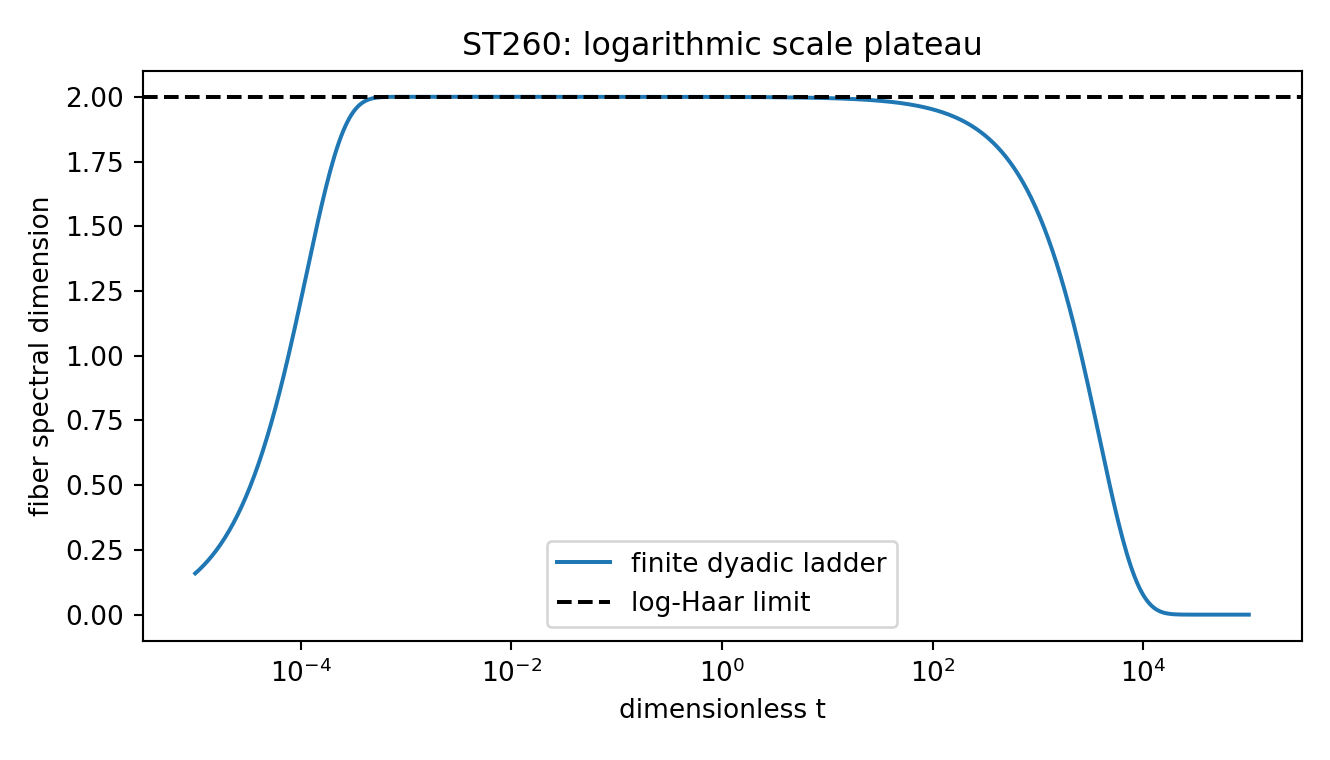
\includegraphics[width=.83\textwidth]{FIN_ST248_ST262_Figures/st260_log_haar_plateau.png}
\caption{ST260: finite dyadic scale flow and its log-Haar continuum plateau.}
\end{figure}

This is the most direct mathematical realization so far of the intuition that observation
may occur through many self-similar compression layers. It does not identify which layer
we inhabit. The density, finite cutoffs, tensor/trace completion, and a physical mapping
from dimensionless $t$ to seconds or length remain missing. The dyadic illustration is not
a license to transfer legacy octave or $\alpha_{\rm geo}$ roles into the strict kernel.

\section{ST261: which observations can see a deeper refinement?}

Let $R$ embed the coarse space and $S$ embed its orthogonal fiber complement. For every
exact self-adjoint refinement
\[
\widetilde A=RAR^*+SBS^*,
\]
functional calculus gives
\[
e^{-t\widetilde A}R=Re^{-tA},\qquad
S^*e^{-t\widetilde A}S=e^{-tB}.
\]

\begin{theorem}[Coarse blindness and complement tomography]
Every experiment whose preparations lie in $\operatorname{Ran}R$ and whose effects are
coarse-compressed is exactly independent of $B$. Conversely, a complement-resolving
preparation and measurement reconstruct $e^{-tB}$. At one known $t>0$,
\[
B=-\frac1t\log\bigl(S^*e^{-t\widetilde A}S\bigr)
\]
is unique.
\end{theorem}

For complement rates $\mu=0.3,1,4$, all coarse return probabilities agree to
$10^{-15}$, while the odd-fiber returns are $e^{-\mu}$ and are plainly separated.

\begin{figure}[H]
\centering
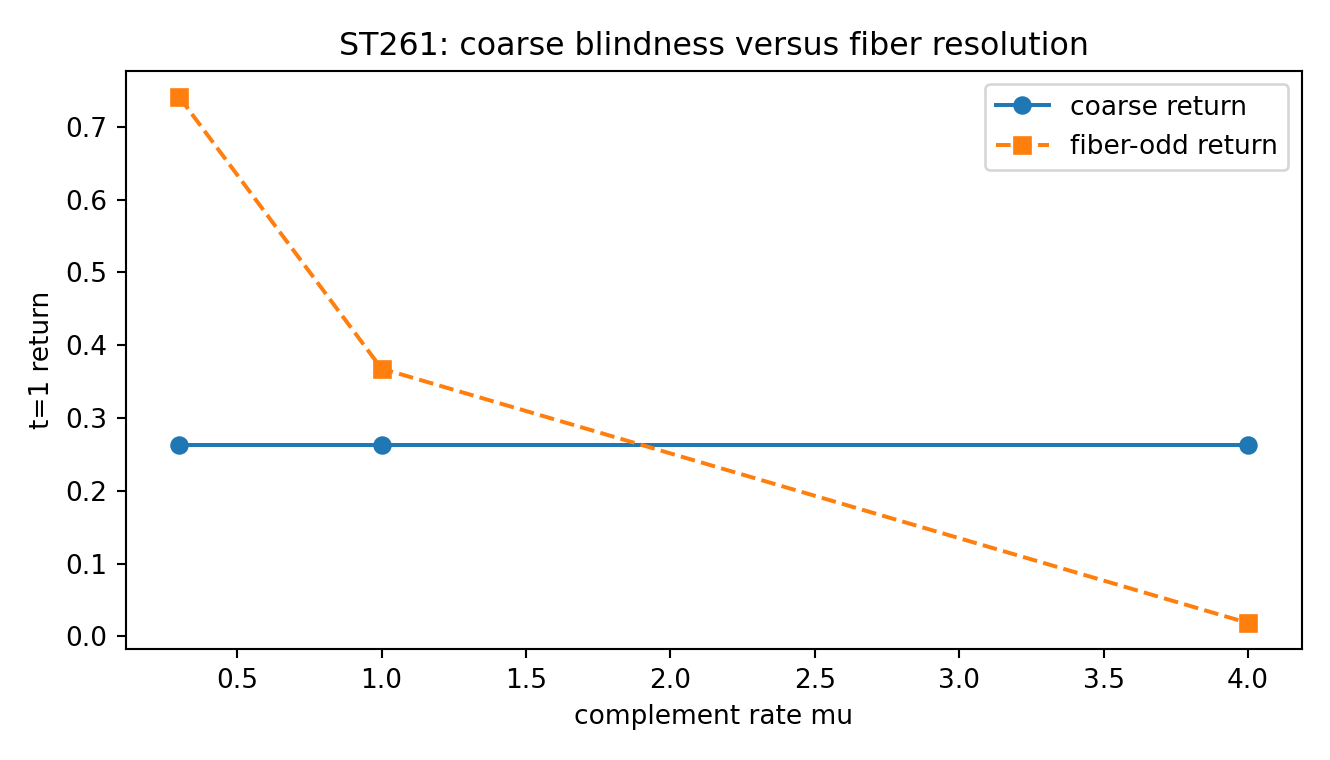
\includegraphics[width=.80\textwidth]{FIN_ST248_ST262_Figures/st261_refinement_observables.png}
\caption{ST261: exact coarse blindness versus complement-sensitive survival.}
\end{figure}

The theorem identifies the missing operational object: a fiber-resolving preparation and
instrument. It does not assert that such a physical fiber exists.

\section{Falsification ledger}

\begin{longtable}{@{}p{0.29\textwidth}p{0.32\textwidth}p{0.30\textwidth}@{}}
\toprule
Candidate claim & Test result & Consequence\\
\midrule
$A$ naturally prepares a localized state & Transitive naturality forces uniform & Strict deterministic preparation source refuted\\
Equivariant filtering creates orientation & Stabilizer can only grow & Input condition carries asymmetry\\
The nonlinear response lacks any repair & Flat quotient connection cancels artifact & Repair exists conditionally on carrier\\
The halfwidth-$0.0005$ cube may lose roots & All 21,952 boxes pass & Prior coarse failures were methodological\\
Finite-sample efficiency is only asymptotic & Explicit modal estimator attains CR exactly & Exact result in declared multinomial model\\
Two marginal gaps solve every joint factor problem & Only aligned two-gap class proved & Generic misalignment remains open\\
Locality selects one refinement & Seven-dimensional positive cone remains & Nonuniqueness reduced, not removed\\
Coarse observations can infer hidden rates & Exact intertwining erases all $B$ dependence & Fiber-resolving instruments are necessary\\
Self-similar rates can form no stable plateau & Log-Haar integral is constant & Plateau shape proved, source not proved\\
Local computation supplies physical evidence & No external record exists & ST262 remains blocked\\
\bottomrule
\end{longtable}

\section{Interpretation for FIN and layered observation}

The combined ST248--ST261 picture is internally coherent. The strict generator determines a
symmetric semigroup and a positive quotient geometry. A localized state creates a second
noncommuting algebra, but cannot be obtained by a deterministic natural rule from $A$
alone. Refinement introduces complement dynamics invisible to every coarse experiment. A
fiber-resolving instrument can reveal them. A log-Haar distribution of fiber rates creates
a broad scale-invariant plateau.

This supports a precise version of the ``observation through fractal layers'' hypothesis:
coarse observers can be exactly blind to complement dynamics while a logarithmic hierarchy
produces approximately scale-independent spectral behavior. It does not establish that
our observed physics is located at a particular layer, nor that deeper scales are physical
lengths. Those conclusions require an operational preparation, a clock and length
calibration, an instrument, and empirical data.

Symmetry remains a reservoir of equivalent possibilities, not positive feedback by itself.
Feedback requires an instability or gain law. ST248 proves that deterministic equivariance
cannot pick one vertex; a genuine spontaneous state source would have to lie outside that
class and still explain its outcome probabilities and orientation.

\section{Recommended programs ST263--ST277}

\begin{enumerate}
\item[\textbf{ST263}.] Test one genuinely new strict symmetry-breaking state source outside
deterministic $D_{12}$-natural rules, or preserve the ST248 no-go.
\item[\textbf{ST264}.] Classify nonlinear equivariant state-to-multiplication maps by orbit
type and stabilizer monotonicity.
\item[\textbf{ST265}.] Extend only the lowest-clearance branch pair with interval event
detection.
\item[\textbf{ST266}.] Derive a rational dual for an affine qubit channel not unitarily
equivalent to amplitude damping or a Pauli mixture.
\item[\textbf{ST267}.] Build an interval KKT certificate or counterexample for ST252.
\item[\textbf{ST268}.] Test uniqueness of the flat mean-zero connection under a wider
naturality category including refinements.
\item[\textbf{ST269}.] Seek the first certified nuisance-cover failure beyond halfwidth
$0.0005$ under a fixed resource cap.
\item[\textbf{ST270}.] Construct exact finite-confidence regions for ST255 under clustered
counts.
\item[\textbf{ST271}.] Resolve generic misaligned joint Clifford uniqueness or give an
explicit two-gap counterexample.
\item[\textbf{ST272}.] Refine the belief-transfer enclosure with adaptive boxes and
optimized Chernoff $s$.
\item[\textbf{ST273}.] Add a finite-dimensional controller and account for its cyclic
free-energy cost.
\item[\textbf{ST274}.] Intersect the ST259 cone with a strict refinement functor only if a
new one is justified.
\item[\textbf{ST275}.] Derive finite-cutoff error bounds for the log-Haar plateau and audit
trace-class completion.
\item[\textbf{ST276}.] Design a frozen fiber-resolving instrument specification without
claiming laboratory execution.
\item[\textbf{ST277}.] Resume external validation only with independently registered
events, calibration, and custody.
\end{enumerate}

The scientific priority is ST263. The present batch has proved exactly why the localized
state cannot be concealed in the symmetric operator. A next attempt is admissible only if
it introduces a genuinely new symmetry-breaking source class. ST275 is the highest-value
multiscale follow-up because it tests whether the log-Haar plateau survives a mathematically
controlled infinite-refinement completion.

\section{Reproducibility}

The executable source \texttt{fin\_st248\_st262\_research.py} writes the aggregate JSON,
CSV ledger, fifteen packets, and eight figures. The replay
\texttt{test\_fin\_st248\_st262.py} checks packet hashes, live representation dimensions,
all 360 continuation inclusions, rational recovery data, the complete 21,952-box count,
exact modal covariance, Clifford excess identity, transfer bounds, graph-Laplacian signs,
and complement observables. The aggregate JSON records Python 3.12.3, NumPy 1.26.4,
SciPy 1.17.1, SymPy 1.12, and random seed \texttt{20260812}.

ST252 is explicitly numerical. ST248, ST249, ST251, ST253--ST261 are theorem-level only
inside their declared mathematical classes. The SHA-256 manifest fixes the release
artifacts byte-for-byte.

\section{Final conclusion}

The current round does not turn FIN into experimentally tested physics. It does replace
three vague questions by precise results:
\begin{align*}
&\boxed{\text{localized preparation is impossible from deterministic symmetric }A\text{ alone}},\\
&\boxed{\text{nonlinear response has a flat covariant completion on }H_0},\\
&\boxed{\text{scale-invariant refinement has log-Haar form and plateau }2\rho\ln2}.
\end{align*}

The remaining boundary is equally precise. A state source must break the ST248 class; a
physical refinement must select one point in the ST259 cone and provide a fiber-resolving
instrument; a physical scale flow must source the log-Haar density, cutoffs, and units. No
such source is presently derived. That separation between achieved mathematics and missing
physics is the main scientific outcome of ST248--ST262.

\end{document}
